\documentclass{standalone}
\usepackage{tikz}

\begin{document}
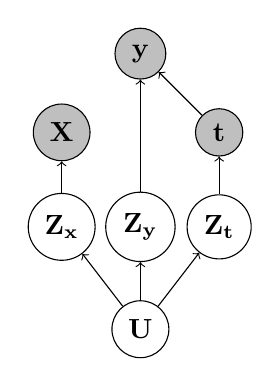
\begin{tikzpicture}
    \node[circle, draw=black, fill=lightgray] (x) at (0, 0) {$\mathbf{X}$};
    \node[circle, draw=black, fill=lightgray] (y) at (1, 1) {$\mathbf{y}$};
    \node[circle, draw=black, fill=lightgray] (t) at (2, 0) {$\mathbf{t}$};
    \node[circle, draw=black, fill=white]     (zx) at (0, -1.2){$\mathbf{Z_x}$};
    \node[circle, draw=black, fill=white]     (zy) at (1, -1.2){$\mathbf{Z_y}$};
    \node[circle, draw=black, fill=white]     (zt) at (2, -1.2){$\mathbf{Z_t}$};
    \node[circle, draw=black, fill=white]     (u) at (1, -2.5){$\mathbf{U}$};
    
    \draw[->] (zx) -- (x);
    \draw[->] (zy) -- (y);
    \draw[->] (zt) -- (t);
    \draw[->] (t) -- (y);
    \draw[->] (u) -- (zx);
    \draw[->] (u) -- (zy);
    \draw[->] (u) -- (zt);
\end{tikzpicture}
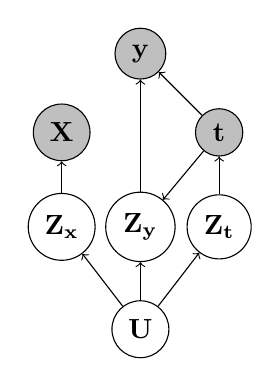
\begin{tikzpicture}
    \node[circle, draw=black, fill=lightgray] (x) at (0, 0) {$\mathbf{X}$};
    \node[circle, draw=black, fill=lightgray] (y) at (1, 1) {$\mathbf{y}$};
    \node[circle, draw=black, fill=lightgray] (t) at (2, 0) {$\mathbf{t}$};
    \node[circle, draw=black, fill=white]     (zx) at (0, -1.2){$\mathbf{Z_x}$};
    \node[circle, draw=black, fill=white]     (zy) at (1, -1.2){$\mathbf{Z_y}$};
    \node[circle, draw=black, fill=white]     (zt) at (2, -1.2){$\mathbf{Z_t}$};
    \node[circle, draw=black, fill=white]     (u) at (1, -2.5){$\mathbf{U}$};
    
    \draw[->] (zx) -- (x);
    \draw[->] (zy) -- (y);
    \draw[->] (zt) -- (t);
    \draw[->] (t) -- (y);
    \draw[->] (u) -- (zx);
    \draw[->] (u) -- (zy);
    \draw[->] (u) -- (zt);
    \draw[->] (t) -- (zy);
\end{tikzpicture}

\end{document}